\documentclass[../main.text]{subfiles}
\begin{document}
\subsection{Quantitative}

Many multivariate visualizations treat the data space as a graph where the vertices's are the variables and the edge corresponds to some quantified relationship between the two vertexes and often these edges are colored by category or form a shape that can be used a proxy for a category. These types of visualizations can often be used to derive typical observations in a given category.

\subsubsection{Parallel Coordinate Plots}
\begin{figure}
  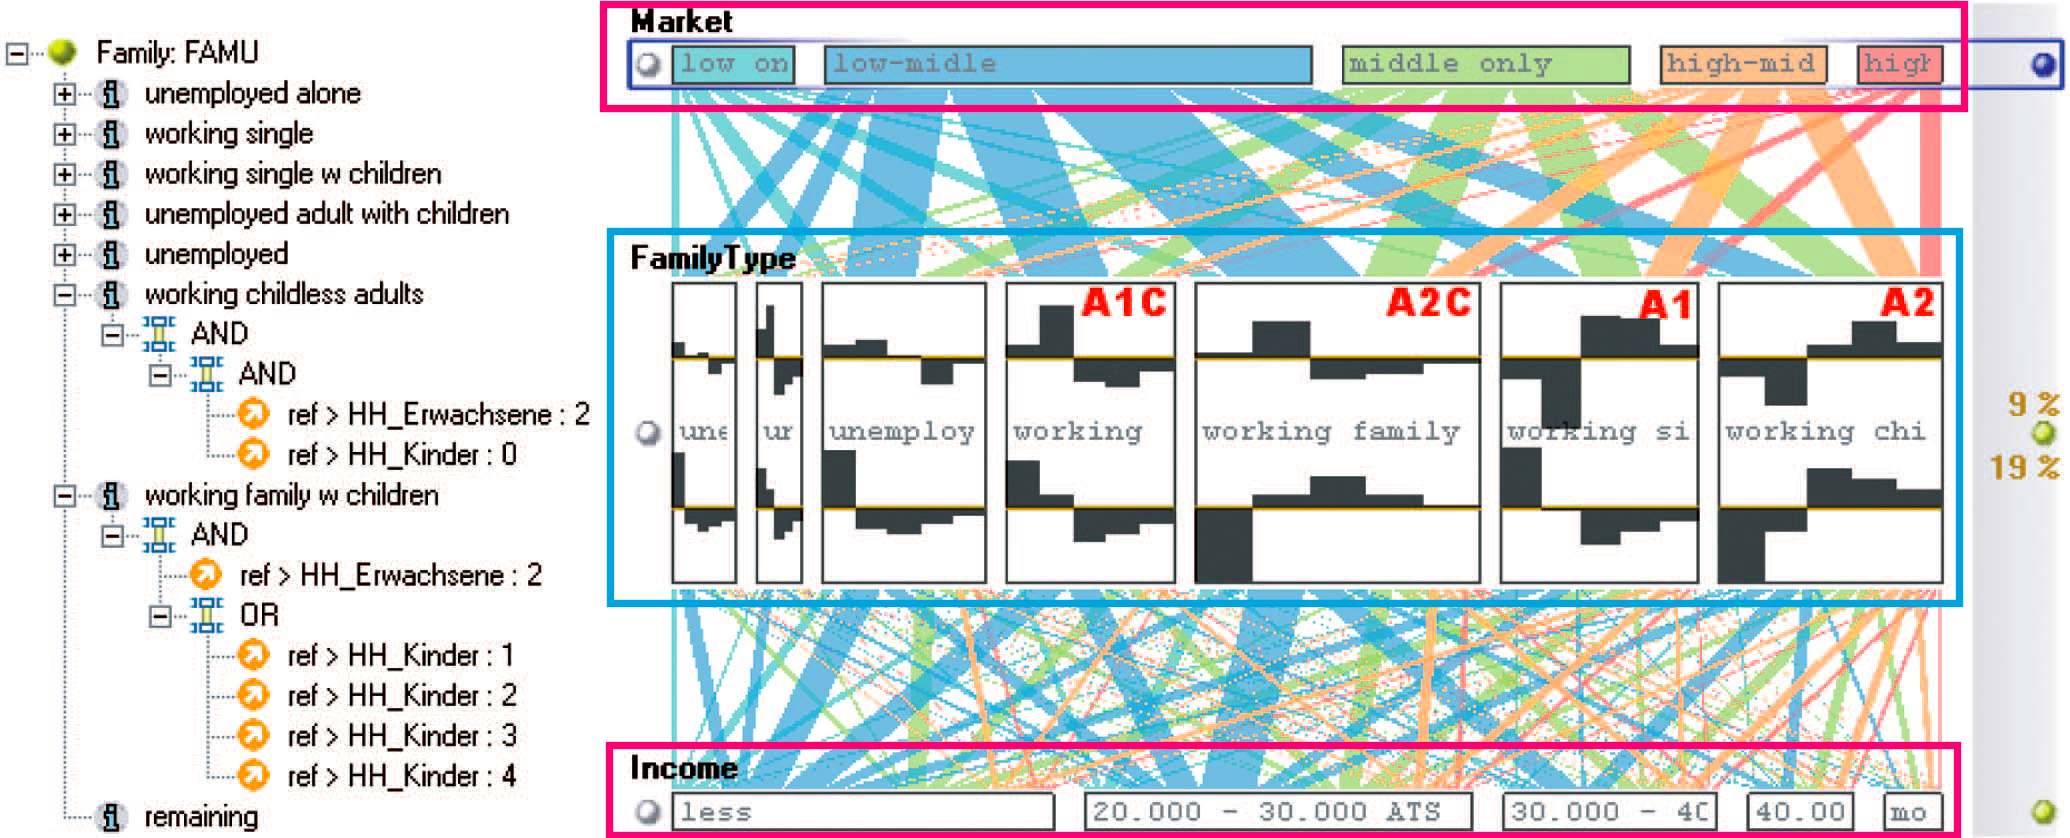
\includegraphics[width=\textwidth]{parallelsets.png}
  \caption{On the left is the categorical view, where users can define
    categories based on other categorical information. For example, in this
    view a working family with children is defined as a household with one or
    more children. On the right is a parallel coordinate graph where the
    dominant category informs the colors, the size of the box is relative to
    the category size, and the histograms show the frequencies of those
    categories relative to the connecting categories (supermarket type and income
    respectively). Because it provides a filtering tool, parallel sets can be used to query whether supermarket and income are conditionally dependent on categorical subsets of family types. This figure is taken from Parallel sets: Interactive exploration and visual analysis of categorical data \cite{kosara_parallel_2006}}
  \label{fig:parallelsets}
\end{figure}

Another important factor in visualizing categorical data is retaining the
inherent hierarchy in many datasets with categorical measurements
\cite{shneiderman_visualizing_2000}. The Parallel Sets tool
shown in figure~\ref{fig:parallelsets} is explicitly designed to show frequencies
of set membership in hierarchal ordered categorical sets \cite{kosara_parallel_2006}. Building on the flexible linked axis version of the parallel coordinates plot \cite{claessen_flexible_2011}, Parallel Sets
  treats each categorical set independently but indicates conditional
  dependency through cross tabulations and by grouping the data. This is indicated via
  color and is based on an active subcategory that then becomes the grouping variable for the
  cross tabulations. In Parallel Sets, quantitative data is converted to
  categorical data via binning. Parallel Sets provides a robust filtering interface for users to test out how different subsets of family type affect their choice in supermarket or their income, which in turn can be used to explore whether there is a conditional dependency amongst these variables. Many-to-many parallel coordinate plot is another type of generalized parallel coordinates where all possible pairs are explored \cite{lind_many--many_2009}.  

\subsubsection{Partial Dependency Plot}

\begin{figure}
    \begin{subfigure}{\textwidth}
    \centering
      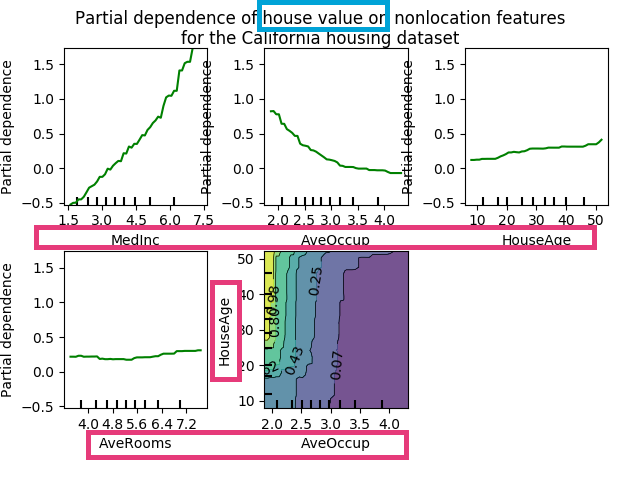
\includegraphics[scale=0.5]{partial_dependence}
      \label{fig:fivechart}
    \end{subfigure}

    \bigskip
    \begin{subfigure}{\textwidth}
    \centering
    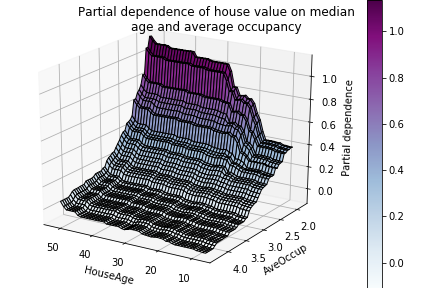
\includegraphics[scale=0.5]{partial_dependency_3}
    \label{fig:threechart}
    \end{subfigure}

  \caption{Taken from Scikit Learn\cite{_partial_????}, the line plots in figure~\subref{fig:fivechart} how California housing prices are partially dependent on each x variable and the joint probability of the variables on housing costs. Figure~\subref{fig:threechart} illustrates the specific relationship between  of the age the house and the number of occupants in the house and the cost.}
  \label{fig:partialdependence}
\end{figure}

One of the most straightforward ways to show dependencies is to plot one
variable against another, but those methods often exclude the effects of the
other variables in the datasets. Regression methods can be used to analyze the
ways in which one variable is partially dependent on many other variables in
the dataset\cite{_elements_2009,scikit-learn}. As shown in figure~\ref{fig:partialdependence}, one way partial dependence line plots and two way partial dependence heat maps and surface maps show how California housing prices are marginally dependent on each variable. While marginal dependence does not directly map to conditional dependence, it establishes that there's a probabilistic relationship between housing prices and median income, average number of occupants, and the age of the house. These variables are then explored further in the heatmap which pinpoints that the marginal probabilities between house age and occupancy are for older houses with few people. Because price can not really affect age, it can be inferred that price is either dependent on age or both are correlated with a third variable. In effect partial dependence plots are computing partial conditional dependencies since they show the probabilistic dependence between a target function and a set of target features. The target features are any set of discrete observations, and the target function is a modeling of a continuous observation. 

\end{document}